\section{Ontologias}

A linguagem está presente na nossa sociedade e na própria constituição do homem.
Ela evolui diariamente e sua complexidade está diretamente associada com todas as
construções do homem, incluindo a Web. Neste contexto de evolução da Web e tecnologia de
informação, ontologia pode ser definida como “a ciência que estrutura e arranja
sistematicamente unidades do conhecimento (os conceitos) de acordo com os elementos de
conhecimento (características) comuns” (DAHLBERG, 2006). Essa, entretanto, pode ser
considerada uma definição simplista, pois está enquadrada apenas no campo da ciência da
informação, de forma que o conceito pode ser expandido em diferentes áreas do
conhecimento \cite{nascimento07} sem se contrapor, dependendo da sua aplicação.

\begin{figure}[!htb]
 \centering
 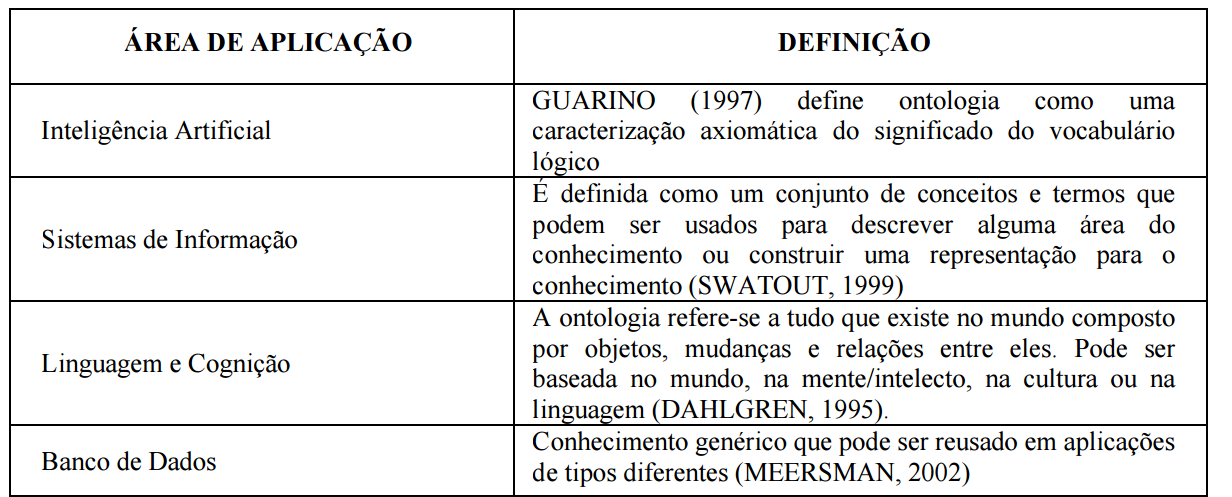
\includegraphics[scale = 0.3]{definicao_ontologias}
 \caption[Diferentes definições de ontologias]{Diferentes definições de ontologias. Fonte: \cite{vitorino06}.}
 \label{fig:definicao_ontologias}
\end{figure}

No que tange ao contexto do nosso projeto, os conceitos aplicados na ciência da
informação e de sistemas de informação são satisfatórios e sustentam a aplicabilidade das
técnicas e frameworks adotados.

De forma geral, podemos admitir que as ontologias são uma especificação explicita de
uma conceituação, ou seja, a definição explicita de conceitos e suas relações, propriedades e
restrições expressas formalmente \cite{gruber93}. Ela permite especificar uma visão
abstrata e simplificada de determinado assunto que se deseja abordar.

O conceito, por sua vez, é compreendido como uma “unidade de conhecimento”
(DAHLBERG, 2006), uma entidade que alimenta a construção de vocabulários e tesauros,
dando subsídio à criação de uma ontologia. Sua aplicação prática é compor as ontologias de
classes e instâncias e mesmo relacionamentos.